\lab{Speech Recognition using CDHMMs}{Speech Recognition using CDHMMs}
\objective{Understand how speech recognition via CDHMMs works, and implement a simplified speech recognition system.}

\section*{Continuous Density Hidden Markov Models}
Some of the most powerful applications of hidden Markov models, speech and voice recognition, result from allowing the observation space to be continuous instead of discrete.
These are called \emph{continuous density hidden Markov models} (CDHMMs).
The two most common formulations are \emph{Gaussian HMMs} and \emph{Gaussian mixture model HMMs} (GMMHMMs).
In this lab, we will focus on GMMHMMs.

A GMMHMM is an HMM where the observation sequence variables $(Z_t)_{t=0}^\infty$ are distributed according to a Gaussian mixture model.
To review, a Gaussian mixture model is a continuous multivariate distribution composed of $K$ Gaussian distributions $\mathcal N(\mu_k,\Sigma_k)$ (where $\mu_k\in \mathbb{R}^M$ and $\Sigma_k\in \mathbb{R}^{M\times M}$) with corresponding weights $c_k$, for $1\leq k \leq K$.
A useful way to think of an individual GMM $Z$ is to think of it as a pair of random variables $Y$ and $Z$.
The variable $Y$ is a categorical variable on $\{1,2,\ldots, K\}$ with probabilities given by the $c_k$ (i.e. $P(Y=k)=c_k$) and determines which Gaussian $Z$ is drawn from.
We then draw $Z\sim \mathcal N(\mu_Y, \Sigma_Y)$.
The density function of a GMM is given as
\[
f(\mathbf{z})=\sum_{k=1}^K c_k\mathcal N(\mathbf{z};\,\mu_k,\Sigma_k).
\]
For an example of what this looks like, refer to Figure \ref{fig:mixture}.
Note that this is a weighted sum of the density functions of Gaussian variables; remember that this is different from a sum of independent Gaussian random variables, which is just another Gaussian random variable!

\begin{figure}
\centering
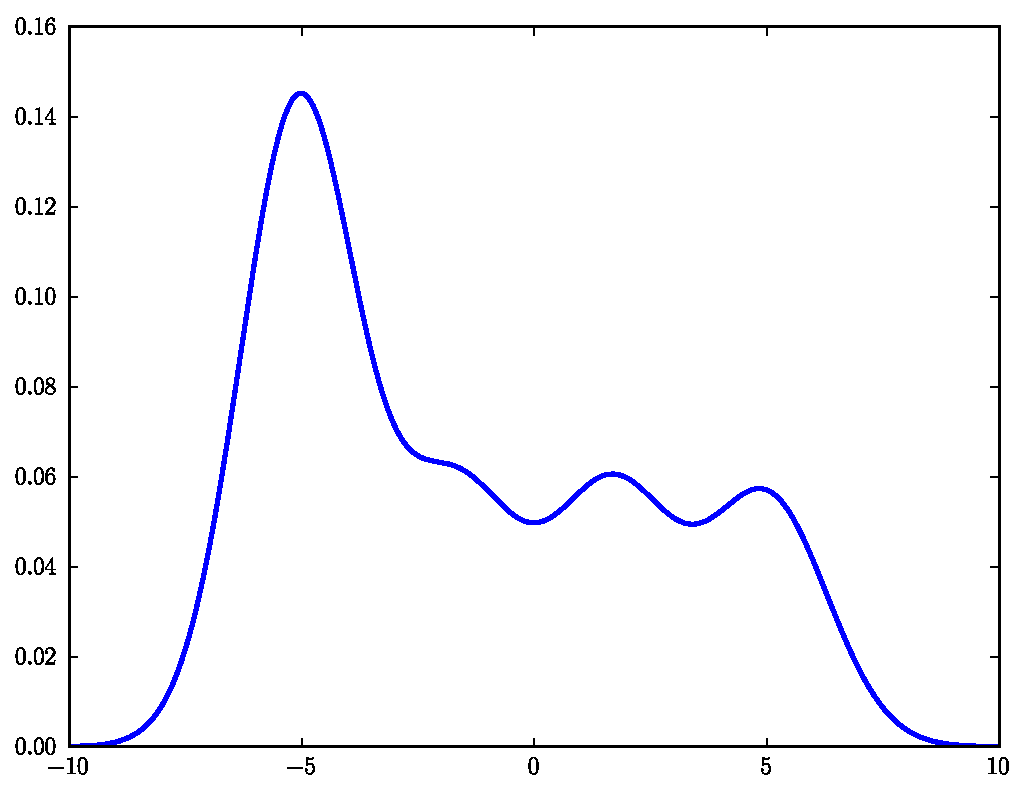
\includegraphics[width=0.6\textwidth]{figures/mixture.pdf}
\caption{The probability density function of a mixture of Gaussians with four components.}
\label{fig:mixture}
\end{figure}

GMMHMMs are then formulated similar to the discrete HMMs we have encountered before.
We will assume that the hidden states $X_t$ have $N$ possible values.
Then, the hidden state of the GMMHMM is parameterized by an initial state vector $\boldsymbol\pi \in \mathbb{R}^N$ and a state transition matrix $A\in \mathbb{R}^{N\times N}$ (both of these are the same as in the discrete case).
The observation state is parameterized by one GMM per hidden state. 
We denote these as follows: for each hidden state $1\leq i \leq n$, the observation state is distributed according to the GMM with component weights $\{c_{i,1},\ldots,c_{i,K}\}$, component means $\{\mu_{i,1},\ldots,\mu_{i,K}\}$, and component covariance matrices $\{\Sigma_{i,1},\ldots,\Sigma_{i,K}\}$.

To sample from a GMMHMM, follow the following process for each time step:
\begin{itemize}
\item Determine the hidden state $X_t$ (for $X_0$ this is with $\boldsymbol\pi$, and afterwards is determined by $A$ and $X_{t-1}$).
\item Determine the GMM component $Y_t$ by drawing from a categorical variable with probabilities $c_{X_t,1},\ldots,c_{X_t,K}$ (so $P(Y_t=j)=c_{X_t,j}$).
\item Sample $Z_t$ from the GMM by drawing from the normal distribution $\mathcal N(\mu_{X_t,Y_t}, \Sigma_{X_t,Y_t})$.
\end{itemize}
For an example of a sequence drawn from a GMMHMM, refer to Figure \ref{fig:samples}, which shows an observation sequence generated from a GMMHMM with two mixture component and two hidden states.

\begin{figure}
\centering
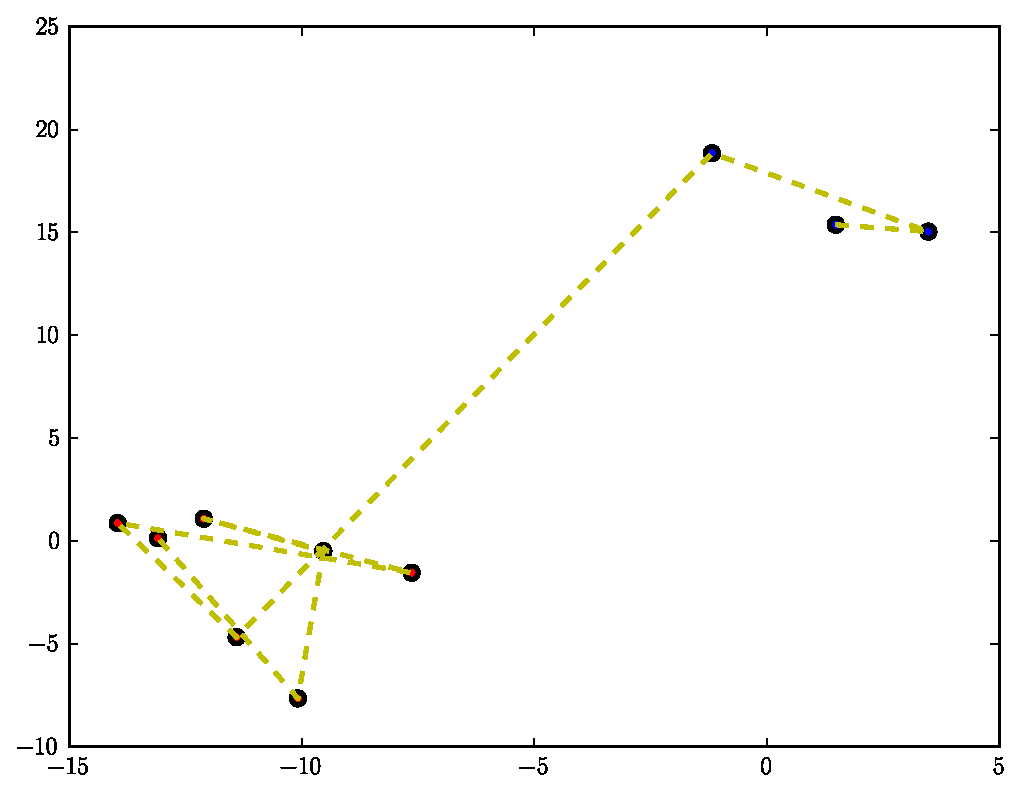
\includegraphics[width=0.6\textwidth]{figures/samples.pdf}
\caption{An observation sequence generated from a GMMHMM with two mixture components and two states.
The observations (points in the plane) are shown as solid dots, the color indicating from which
state they were generated. The connecting dotted lines indicate the sequential order of the observations.}
\label{fig:samples}
\end{figure}

\begin{problem}
Consider the following GMMHMM with $N=3$ states, components of dimension $M = 4$, and $K=5$ components:
\begin{lstlisting}
# NxN transition matrix 
A = np.array([[.3, .3, .4], [.2, .3, .5], [.3, .2, .5]])
# NxK collection of component weights
weights = np.array([[.3, .2, .1, .2, .2], [.1, .3, .3, .2, .1], 
                    [.1, .3, .2, .1, .3]])
# NxKxM collection of component means
means = np.array([np.floor(np.random.uniform(-100, 100, size = (5, 4))) 
                        for i in range(3)])
# NxKx(MxM) collection of component covariance matrices       
covars = np.array([[np.floor(np.random.uniform(1, 20))*np.eye(4) 
                        for i in range(5)] for j in range(3)])
# (N,) ndarray initial state distribution 
pi = np.array([.15, .15, .7])
\end{lstlisting}
The weight $c_{i,k}$ is \li{weights[i,k]}, the mean $\mu_{i,k}$ is \li{means[i,k,:]}, and the covariance matrix $\Sigma_{i,k}$ is \li{covars[i,k,:,:]}.

Write a function \li{sample_gmmhmm} which accepts an integer $T$, and draws $T$ samples from the above GMMHMM.

Use your function to draw $T=900$ samples.
Use \li{sklearn.decomposition.PCA} with 2 components to plot the observations in two-dimensional space. 
Color the observations by state.
How many distinct clusters do you see?

Hint: the function \li{np.random.choice} will be useful for drawing the hidden states and the GMM components, and \li{np.random.multivariate_normal} for the observation sequence. 
When plotting the samples, using the keyword argument \li{c} in \li{plt.scatter} allows you to specify the colors of the individual points.
\end{problem}

\section*{Speech Recognition and Hidden Markov Models}
The questions we asked about discrete HMMs can also be asked about CDHMMs, and the algorithms that answer these questions are virtually identical to the discrete case.
However, with continuous observations it is much more difficult to implement the algorithms in a numerically stable way.
We will not have you implement any of the algorithms for CDHMMs yourself; instead, we will use the \li{hmmlearn} package.

Hidden Markov Models are the basis of modern speech recognition systems.
The essential idea is that we will use the sound data as the observation sequence.
However, there are a lot of details that we won't address in this lab; a fair amount of signal processing must precede the HMM stage, and more sophisticated approaches require the use of language models.

To transform the audio data into data for our HMMs, we will use the following process:
\begin{itemize}
\item Divide the audio into frames of approximately 30 ms. These are short enough that we can treat the signal as being constant over these intervals. 
\item Transform the audio signal into mel-frequency cepstral coefficients (MFCCs). This transformation is similar to a Fourier transform in that it breaks the sound signal into frequencies. 
\item Keep the first $M=10$ of these coefficients for each time frame. These will be our observation sequence in $\mathbb{R}^M$.
\end{itemize}

\begin{problem}
In the remainder of this lab, we will create a speech recognition system for the vocabulary of the following five words/phrases: ``biology'', ``mathematics'', ``political science'', ``psychology'', and ``statistics''.

The \li{Samples} folder contains 30 recordings for each of the words/phrases in the vocabulary.
These audio samples are 2 seconds in duration, recorded at a rate of 44100 samples per second, with samples stored as 16-bit signed integers in WAV format. 
For each of the words, create a list holding the MFCC coefficients of the recordings of that word.

The function \li{scipy.io.wavfile.read} can be used to load the sound files, and the function \li{extract} in \li{MFCC.py} implements the MFCC coefficient algorithm:
\begin{lstlisting}
from scipy.io import wavfile
import MFCC

samplerate, sound_data = wavfile.read(filename)
coefficients = MFCC.extract(sound_data)
\end{lstlisting}
Hint: it might be helpful to use a dictionary to store the lists of coefficients.
\end{problem}

Industrial-grade speech recognition systems train a GMMHMM for each individual English \emph{phoneme}, or distinct sound.
This allows for a lot of versatility, but also comes with its own set of challenges: it requires a lot of training data, with the audio files split into individual phonemes, as well as requiring the true words to be written in terms of their phonemes.
The setup also becomes much more complicated if we try to account for multiple dialects of English.

Instead, in this lab, we will train a GMMHMM for each of the five individual words in the vocabulary.\footnote{For a larger vocabulary, this requires a ludicrous number of GMMHMMs, which is why speech recognition systems don't typically do this.}
Recall, however, that the training procedure can get stuck in a poor local minimum. 
To combat this, we will train 10 GMMHMMs for each word (using a different random initialization of the parameters each time)
and keep the model with the highest log-likelihood.

For training our HMM, we will use the \li{hmmlearn.hmm.GMMHMM} class.
We will illustrate how to use this class.
Let \li{data} be a list of arrays, where each array is the output of the MFCC extraction for a speech sample.
Then the model can be trained as follows:

\begin{lstlisting}
import numpy as np
from hmmlearn import hmm

# hmmlearn expects the data to be in a single array:
data_collected = np.vstack(data)
# To separate the sequences, it requires the length of each:
lengths = [item.shape[0] for item in data]

# Initialize and train the model
model = hmm.GMMHMM(n_components=5, covariance_type="diag")
model.fit(data_collected, lengths=lengths)

# Check the log-likelihood
log_likelihood = model.monitor_.history[-1]
\end{lstlisting}

\begin{problem}
For each word, randomly split the list of MFCCs into a training set of 20 samples and a test set of the remaining 10 samples.

Use the training sets to train GMMHMMs on each word in the vocabulary.
For each word in the vocabulary, train 10 GMMHMMs on the training set, using \li{n_components=5}.
Keep the model with the highest log-likelihood for each word.
\end{problem}

We have now trained our speech recognition system.
With this model, if we are given a speech sample, how do we determine which word it is?

The method we use is as follows. 
First, we convert the sound into MFCC coefficients.
Let $\mathbf{z}$ denote these coefficients.
Then, for each of the words in our vocabulary, we find $\log P(\mathbf{z}\,|\,\text{word})$, the log probability density of this observation sequence assuming that it came from that word's GMMHMM.
This can be done with the \li{score} method of the \li{GMMHMM}.
Then, whichever word's GMMHMM gives the highest log probability density will be our speech recognition model's prediction.

\begin{problem}
Write a \li{predict} function for your speech recognition model.
In this function:
\begin{itemize}
\item Accept the MFCC coefficients of the speech sample to be predicted.
\item Find the log probability density of the coefficients for each word's GMMHMM.
\item Return the word with the highest probability as the speech recognition model's prediction.
\end{itemize}
\end{problem}

\begin{problem}
For each of the five test sets, call your \li{predict} function on each sample, and find the proportion of each test set that your model predicts correctly.
Display your results.
How well does your model perform on this dataset?
\end{problem}